\section{Introduction}

The aim of this project is to investigate the practical use of photogrammetry,
with a focus of its applications to the Earth Sciences. It covers the methods
used to gain photogrammetric data and analyses some results taken from
fieldwork.

\subsection{How photogrammetry works}

The basic principle of photogrammetry is the same mechanism by which the eyes
infer distance: triangulation. By moving around an object, or parallel to a
façade, one can infer the distance to the object by a simple trigonometric
calculation, as demonstrated in Figure \ref{fig:triangulation}. By leveraging
this simple trigonometric distance calculation, one can infer from the group of
photos of the same object, taken using the appropriate method as described in
Section \ref{sec:methods/photographic-technique}, the distance to any point in
the photos, and thus built up a three dimensional model of the captured objects.
Importantly, this can be achieved without need for explicitly inputting the
location that the photographs were taken, although it does increase the accuracy
of the resulting model, as discussed in Section \ref{sec:methods/geotagging}.

\begin{wrapfigure}{r}{0.5\textwidth}
    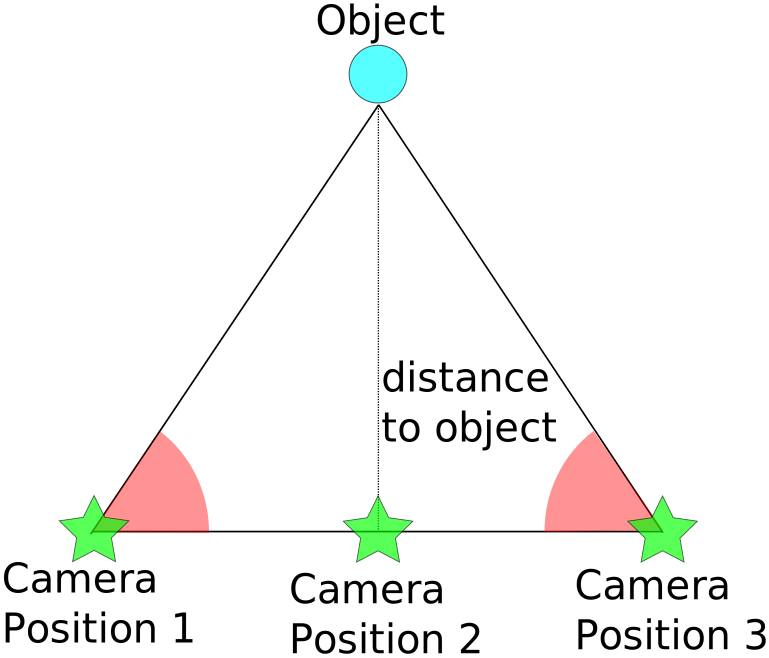
\includegraphics[width=\linewidth]{Triangulation}
    \caption{By taking photographs of an object from different angles, one can
        use trigonometry to calculate the distance to that object.}
    \label{fig:triangulation}
    \vspace{-30pt}
\end{wrapfigure}

\subsection{Unmanned Aerial Vehicles}

To gain the photographs and geopositioning data for the photogrammetric
reconstruction, we employ the use of Unmanned Aerial Vehicles (UAV). To this
end, the ArduPilot Mega (APM)\footurl{http://www.ardupilot.co.uk/} autopilot
on-flight hardware and firmware is used.  Although a quadcopter is the focus of
the research, data was also taken with a hexacopter.

\subsection{Software Used}

\subsubsection{Mission Planner}

Mission Planner\footurl{http://planner.ardupilot.com} was used to interact with
and give commands to the APM autopilot. In particular the \texttt{survey grid}
option, used to guide the UAV in a regular grid pattern, is useful for achieving
successful photos for modelling. In addition, Mission Planner is used to geotag
the photos. This is discussed in more detail in \ref{sec:methods/geotagging}.

\subsubsection{Agisoft PhotoScan}

The Agisoft PhotoScan Professional Edition
software\footurl{http://www.agisoft.ru/products/photoscan/professional/}
software is used to perform the photogrammetric reconstruction. The workflow is
as follows:

\begin{description}
    \item[Load Photos] Firstly, the photos are loaded in PhotoScan.
    \item[Load Camera Positions] Then, the camera geotagging data are loaded,
        either through importing the photo exif metadata, or through a separate
        comma separated value file.
    \item[Align Photos] The camera positions are then used to refine the camera
        position and build a sparse point cloud.
    \item[Place Ground Control Points] Next a mesh is generated and the GCPs are
        input into PhotoScan.
    \item[Optimise alignment] The camera alignment is then optimised using the
        GCP data.
    \item[Build Dense Point Cloud] PhotoScan subsequently builds a dense point
        cloud from the sparse point cloud.
    \item[Build Mesh] Penultimately, the mesh is built by joining the dense
        point cloud into a smooth model.
    \item[Build Texture] Finally, the mesh is overlaid with a texture, finished
        the photogrammetric reconstruction.
\end{description}

Once this workflow is accomplished, the resulting model can be exported as an
orthophoto, whereby the original photos are stitched together into a single
aerial image, and as a Digital Elevation Model (DEM), which contains all the
information about the topography of the model. It is this DEM that is of
application to Earth Science research.

\subsubsection{Canon Hack Development Kit}

In order to control the camera remotely, we employed the Canon Hack Development
Kit (CHDK)\footurl{http://chdk.wikia.com/}. Specifically, we used firmware
version 1.00B Alpha for the Powershot
IXUS132\footurl{http://chdk.wikia.com/wiki/ELPH115}, loaded by a bootable SD
card. This allows one to run scripts on the camera, written in either Lua or
UBASIC, that interface with the camera mechanism, e.g. taking pictures, zooming,
turning off etc. This allowed us control over the camera during the flights.
